\subsection{Database}
The database will be used to keep track of user info which includes name, email, passwords, connections (to different services), user preferences, etc.

\begin{figure}[h!]
	\centering
 	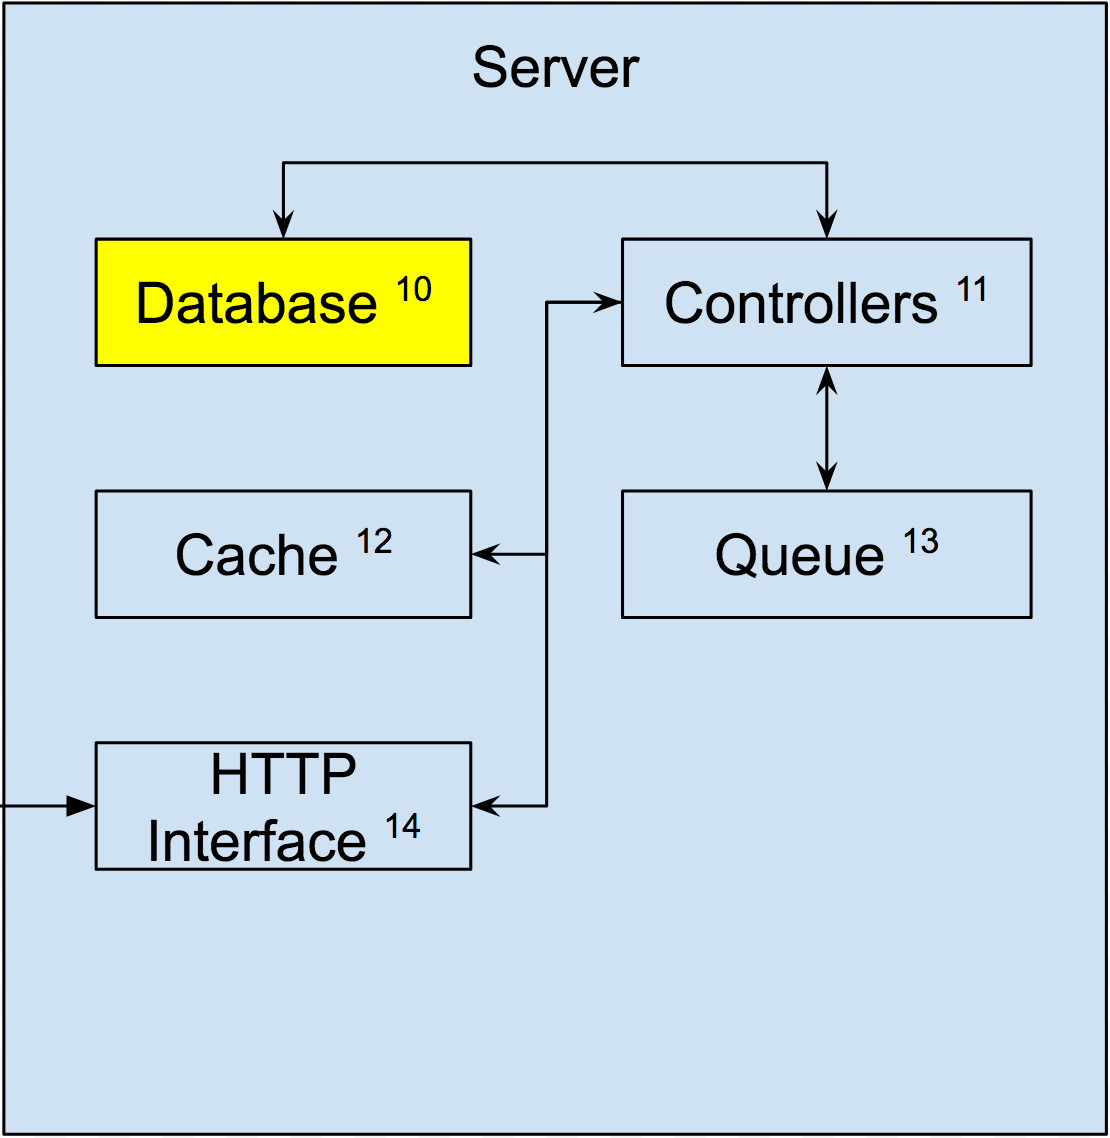
\includegraphics[width=0.60\textwidth]{images/server/server_database.png}
 	\caption{Database subsystem}
\end{figure}

\subsubsection{Assumptions}
N/A

\subsubsection{Responsibilities}
The responsibilities of the database will be to manage user data

\subsubsection{Subsystem Interfaces}
\begin {table}[H]
\caption {Database interfaces} 
\begin{center}
    \begin{tabular}{ | p{1cm} | p{3cm} | p{6cm} | p{6cm} |}
    \hline
    ID & Description & Inputs & Outputs \\ \hline
    \#01 & Store new user & \pbox{6cm}{New user data} & \pbox{6cm}{Confirmation query with new user data saved}  \\ \hline
    \#02 & Returning user login credentials & \pbox{6cm}{Return user e-mail/password} & \pbox{6cm}{Confirmation query with existing user data returned}  \\ \hline
    \end{tabular}
\end{center}
\end{table}

\newpage
